\newpage
\section{The Hydrogen Atom}

\subsection{Mystery of the Hydrogen Atom}

By the early 1900s, scientists understood that matter came in tiny pieces called atoms and that an atom of hydrogen contained charge $+e$ proton at its center and charge $-e$ electron outside that center. 

\begin{figure}[H]
    \centering
    \includegraphics[width=0.309\textwidth]{Lec25/Bohr’s model for hydrogen resembles the orbital model of a planet around a star.}
    \caption{Bohr’s model for hydrogen resembles the orbital model of a planet around a star.}
\end{figure}

Because the proton's mass is much greater than the electron's mass, we shall assume that the \highlight{proton is fixed in place}. So, the atom is a fixed potential trap with the electron moving around inside it. A hydrogen atom contains an electron that is trapped by the Coulomb force it experiences from the proton, which is the nucleus of the atom. Under Newtonian laws, the electron would move around the proton, like planets around the Sun, i.e.,
\begin{align*}
    \frac{1}{4\pi \epsilon_0}\frac{e^2}{r^2}=m\frac{v^2}{r}
\end{align*}
Multiplying by $-r$, we obtain
\begin{align*}
    E_C=-\frac{e^2}{4\pi \epsilon_0 r}=-mv^2=-2E_K
\end{align*}
Alternatively, the total energy of the electron is 
\begin{align*}
    E=E_K+E_C=\frac{E_C}{2}=-E_K
\end{align*}

However, any charged particle which moves in a curved path will emit electromagnetic radiation, hence losing energy continuously. \highlight{Why doesn’t the electrical attraction between the electron and the positive charge simply cause the two to collapse together?}

One clue lay in the experimental fact that a hydrogen atom can emit and absorb only four wavelengths in the visible spectrum (656 nm, 486 nm, 434 nm, and 410 nm).

\subsection{The Bohr Model}
Bohr made two bold (and completely unjustified) assumptions:
\begin{enumerate}
    \item The electron in a hydrogen atom orbits the nucleus in a circle much like Earth orbits the Sun. 
    \item The magnitude of the angular momentum $\vec{L}$ of the electron in its orbit is restricted (quantized) to the values
    \begin{align*}
        L=n\hbar
    \end{align*}
    for $n=1,2,3,\dots$
\end{enumerate}

However, as successful as his theory was on the four visible wavelengths and on why the atom did not simply collapse, it turned out to be quite wrong in almost every other aspect of the atom. We follow Bohr to quantize the electron orbit:
\begin{align*}
    L=rmv=n\hbar
\end{align*}
from which we find $v=\frac{n\hbar}{mr}$. 

Combining with the Newtonian result, we find 
\begin{align*}
    r_n=n^2a_B
\end{align*}
where the characteristic length
\begin{align*}
    a_B=\frac{\hbar^2}{\frac{me^2}{4\pi \epsilon_0}}=0.529\text{\AA}
\end{align*}

In the Bohr model of the hydrogen atom, the electron’s orbital radius r is quantized and the smallest possible orbital radius (for $n = 1$) is $a_B$ , which is called the \highlight{Bohr radius}. According to the Bohr model, the electron cannot get any closer to the nucleus than orbital radius $a_B$ , and that is why the attraction between electron and nucleus does not simply collapse them together.

The energy of the hydrogen atom, according to the Bohr
model, is then
\begin{align*}
    E_n=\frac{1}{2}mv^2-\frac{1}{4\pi \epsilon_0}\frac{e^2}{r}=-\frac{E_R}{n^2}
\end{align*}
where the characteristic energy (known as the \highlight{Rydberg})
\begin{align*}
    E_R=\frac{\frac{me^4}{(4\pi \epsilon_0)^2}}{2\hbar^2}=13.6 \, \text{eV}
\end{align*}
Note that we still have, for each orbit
\begin{align*}
    E=E_K+E_C=\frac{E_C}{2}=-E_K
\end{align*}

\subsubsection{The Hydrogen Spectrum}
The energy of a hydrogen atom (or, equivalently, of its electron) changes when the atom emits or absorbs light.
Emission and absorption involve a quantum of light according to
\begin{align*}
    \hbar \omega_{nm}=E_R\left(\frac{1}{n^2}-\frac{1}{m^2}\right)
\end{align*}
for integers $m>n$. The wavelengths of the emitted or absorbed light are given by
\begin{align*}
    \frac{1}{\lambda}=\frac{E_R}{hc}\left(\frac{1}{n^2}-\frac{1}{m^2}\right)
\end{align*}

The collection of such lines (or wavelengths), such as in those in the visible range, is called a spectrum of the hydrogen atom. For convenience, we often quote the value of the combination $hc=12400$eV\AA . Hence, we have
\begin{align*}
    \frac{hc}{E_R}=912\text{\AA}
\end{align*}

\begin{figure}[H]
    \centering
    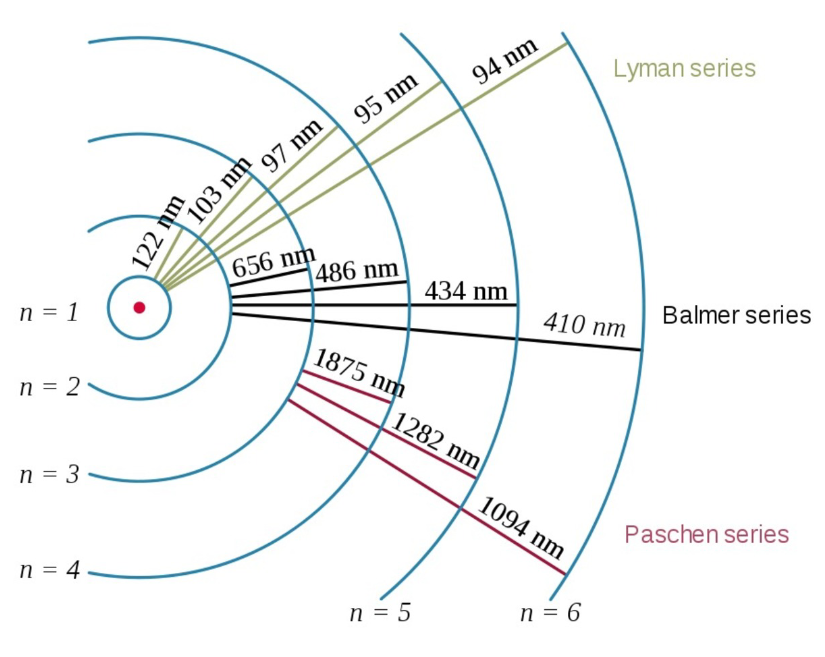
\includegraphics[width=0.309\textwidth]{Lec25/The Hydrogen Spectrum}
    \caption{The Hydrogen Spectrum}
\end{figure}

\subsubsection{Combinations of Physical Constants}
As a side remark, it is often convenient to remember and use combinations of physical constants. Some examples are
\begin{align*}
    h c=&12400 \mathrm{eV} \cdot \text{\AA} \\
    \hbar c=&h c /(2 \pi)=1973 \mathrm{eV} \cdot \text{\AA} \\
    e^{2} /\left(4 \pi \epsilon_{0}\right)=&14.4 \mathrm{eV} \cdot \text{\AA} \\
    k_{B} T_{\text {room }}=&1 / 40 \mathrm{eV} \\
    m_{e} c^{2}=&511000 \mathrm{eV}=0.511 \mathrm{MeV} \\
    m_{p} / m_{e}=&1836
\end{align*}

\subsection{Ground-State Energy from Uncertainty P- rinciple}

The ground-state energy is the lowest energy allowed by Heisenberg’s uncertainty principle. For a hydrogen atom, the size of the wave function, $\Delta r$ , is the uncertainty in position. The uncertainty in momentum is, roughly speaking, $\Delta p \sim \hbar/\Delta r$ , by the uncertainty principle. The energy of the electron can be estimated to be
\begin{align*}
    E\sim\frac{(\Delta p)^2}{2m}-\frac{e^2}{4\pi\epsilon_0 \Delta_r}=\frac{\hbar^2}{2m(\Delta r)^2}-\frac{e^2}{4\pi\epsilon_0 \Delta_r}
\end{align*}
To find the minimal energy, we solve, for $\Delta r$
\begin{align*}
    \frac{\mathrm{d}E}{\mathrm{d}(\Delta r)}=0
\end{align*}
After some algebra, we find
\begin{align*}
    \Delta r=&\frac{\hbar^2}{\frac{me^2}{4\pi\epsilon_0}}\equiv a_B\\
    E=&-\frac{\frac{me^2}{4\pi\epsilon_0}}{2\hbar^2}\equiv -E_R
\end{align*}

The energy of the ground state (or any stationary state) is uniquely determined. This is because of the energy-time uncertainty principle,
\begin{align*}
    \Delta t \cdot \Delta E \ge \hbar/2
\end{align*}
In the extreme case of a stationary state, $\Delta t=\infty$, so we have $\Delta E=0$. Note, however, both kinetic energy and potential energy have uncertainties, due to the uncertainties of position and momentum. 

\subsection{Solutions of Schroedinger’s Equation}
In Schroedinger's model of the hydrogen atom, the electron (charge $-e$) is in a potential energy trap due to its electrical attraction to the proton (charge $+e$) at the center of the atom. 

\begin{figure}[H]
    \centering
    \includegraphics[width=0.309\textwidth]{Lec25/Schroedinger’s Equation for the H-Atom}
    \caption{Schroedinger’s Equation for the H-Atom}
\end{figure}

With the central potential, we can use separation of variables and assume 
\begin{align*}
    \Psi(r,\theta,\phi)=R(r)\Theta(\theta)\Phi(\phi) 
\end{align*}
which breaks the equation into three separate differential equations for $R(r)$, $\Theta(\theta)$ and $\Phi(\phi)$.  

The $\Phi$ function is found to have the quantum number $m$ where
\begin{align*}
    \Phi_{m_l}(\phi)\sim e^{im_l \phi} ,\, m_l=0,\pm 1,\pm 2, \dots
\end{align*}

The $\Theta$ function is known as \highlight{Legendre polynomials}, which have quantum number $m_l$ and $l$. When $\Theta$ and $\Phi$ are multiplied together, the product is known as spherical harmonics
\begin{align*}
    Y_l^{m_l}(\theta,\phi)=\Theta_l^{m_l}(\theta)\Phi_{m_l}(\phi)
\end{align*}

The radial wave function $R_{n,l}(r)$ has quantum number $n$ and $l$. 

\subsubsection{Hydrogen Wave Functions}
The solution for the energy levels is exactly what Bohr found by using the incorrect planetary model of the atom. The corresponding wave function of a particular quantum state of the hydrogen atom can be labeled by a set of quantum numbers $(n,l,m_l)$
\begin{enumerate}
    \item The corresponding energy only depends on the \highlight{principal quantum number} $n=1,2,3,\dots$
    \item The \highlight{orbital quantum number} $l=1,2,3,\dots$ , $n-1$ is a measure of the magnitude of the angular momentum of the quantum state. States with $l = 0, 1, 2, 3$ are called $s, p, d, f$ .
    \item The \highlight{orbital magnetic quantum number} $m_l=-l,-l+1,\dots,l-1$, $l$ is related to the space orientation of this angular momentum vector.
\end{enumerate}

\subsubsection{Ground State Wave Function}
The wave function for the ground state of the hydrogen atom, as obtained by solving the three-dimensional Schroedinger equation and normalizing the result, is
\begin{align*}
    \psi_{100}(\vec{r})=R_{10}(r)=\frac{1}{\sqrt{\pi}a_B^{3/2}}e^{-r/a_B}
\end{align*}
Note that the hydrogen atom in its ground state has zero angular momentum, which is not predicted in the Bohr model. 

\begin{figure}[H]
    \centering
    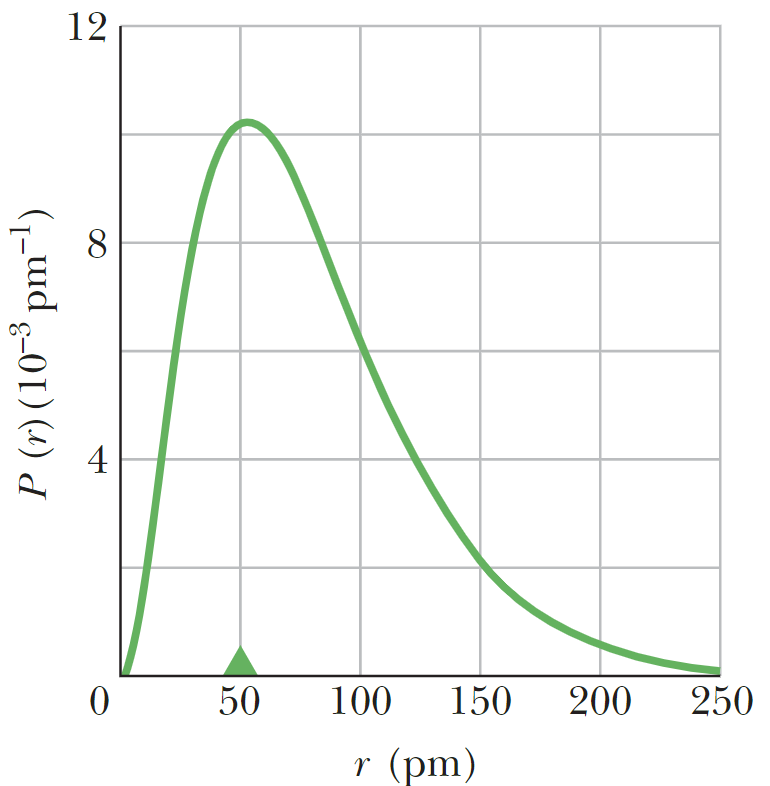
\includegraphics[width=0.309\textwidth]{Lec25/radial probability density}
    \caption{The radial probability density $P(r)$}
\end{figure}


The probability that the electron can be detected in any given (infinitesimal) volume element $\mathrm{d}V$ located at radius $r$ from the center of the atom is $|\psi_{100}(\vec{r})|^2\,\mathrm{d}V$. With spherical
symmetry, we have $\mathrm{d}V=4\pi r^2 \,\mathrm{d}r$. We define \highlight{radial probability density $P(r)$} such that
\begin{align*}
    P(r)\,\mathrm{d}r=|\psi_{100}(\vec{r})|^2\,\mathrm{d}V
\end{align*} 

The popular view that electrons in atoms follow well-defined orbits like planets smoving around the Sun is incorrect. All that we can ever know about the location of the electron in the ground state of the hydrogen atom is the radial probability density. We can show the probabilistic nature of the wave function by a dot plot: The density of dots represents the probability density of detection of the electron with the hydrogen atom in its ground state.

\subsubsection{Bohr’s Correspondence Principle}
The probability density for a hydrogen atom state with a relatively high n and the highest $l = n - 1$ forms a ring that indeed look like a de Broglie wave. The resemblance of the probability density to the electron orbit of classical physics is another illustration of Bohr’s \highlight{correspondence principle} — namely, that at large quantum numbers the predictions of quantum mechanics merge smoothly with those of classical physics

\subsection{The Pauli Exclusion Principle}
For multiple electrons in the same trap, we must consider the Pauli exclusion principle, named after Wolfgang Pauli. The Pauli principle states that no two electrons confined to the same trap can have the same set of values for their quantum numbers. In other words, there can be two electrons at most at any energy level; they have opposite spins. This principle applies not only to electrons but also to protons and neutrons, all of which have $s = 1/2$; they are known as \highlight{Fermions}.

Consider electrons in an infinite square well with side length $L$ (with $E_{n_1,n_2}=n_1^2+n_2^2$, in units of $\frac{h^2}{8mL^2}$). 

\begin{figure}[H]
    \centering
    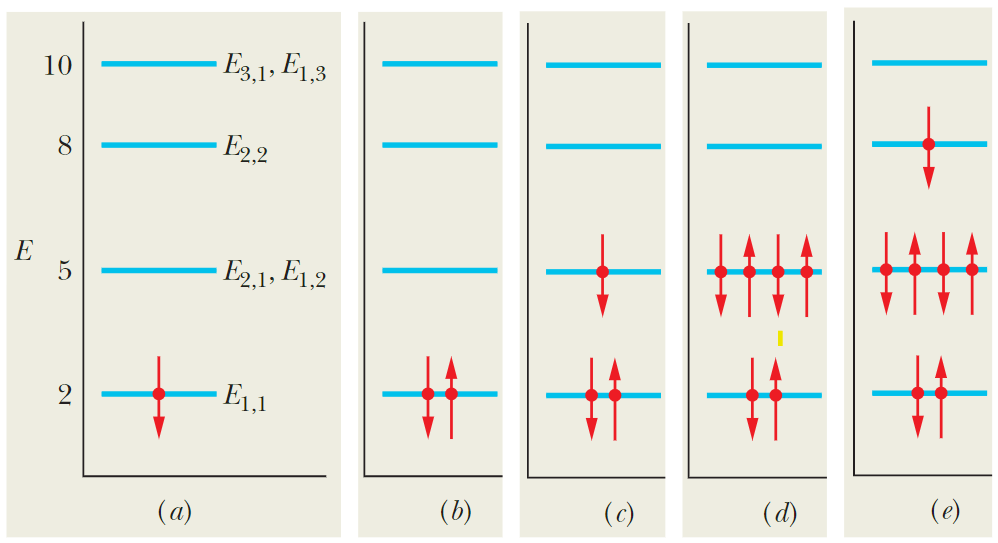
\includegraphics[width=0.42\textwidth]{Lec25/The Pauli Exclusion Principle}
    \caption{The Pauli Exclusion Principle}
\end{figure}

\subsubsection{Carbon}
A carbon atom has a nucleus of 6 protons and 6 neutrons with a total charge of $6e$. The lowest level $(1s)$ contains 2 electrons, one spin up and one spin down. There are 4 electrons on the outer shell [$2s$ (lower in energy) and $2p$].

\begin{figure}[H]
    \centering
    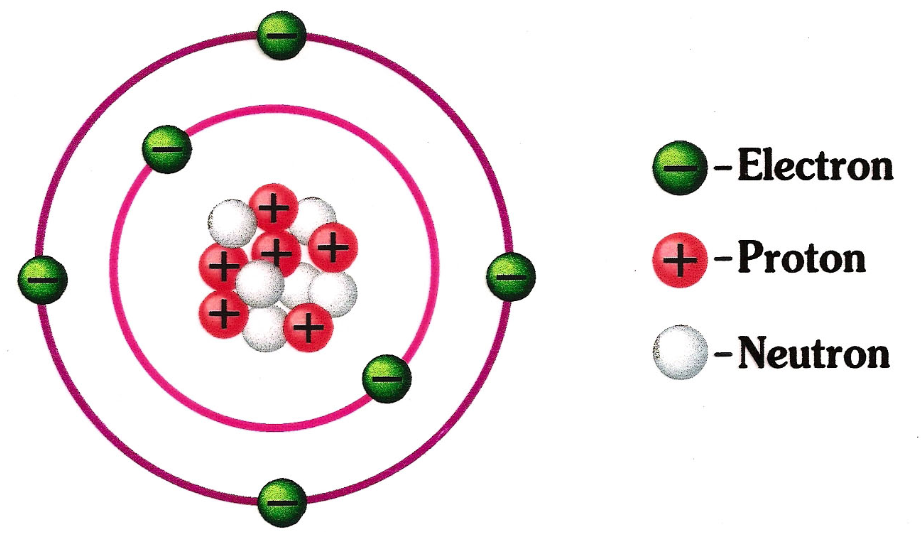
\includegraphics[width=0.309\textwidth]{Lec25/Carbon}
    \caption{Carbon}
\end{figure}

\subsection{Wave Function Hybridization}
Hybridization is the idea that atomic orbitals fuse to form newly hybridized orbitals, which in turn, influences molecular geometry and bonding properties. 

\subsubsection{\texorpdfstring{$sp^3$}. Hybridization}
In menthane, the carbon 2s and 2p orbitals are hybridized.

\begin{figure}[H]
    \centering
    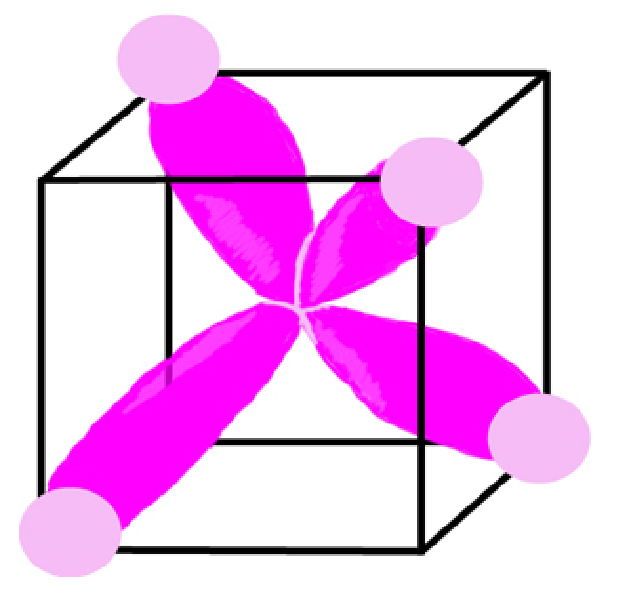
\includegraphics[width=0.22\textwidth]{Lec25/3p3 Hybridization}
    \caption{$sp^3$ Hybridization}
\end{figure}

\subsubsection{\texorpdfstring{$sp^2$}. Hybridization}

\begin{figure}[H]
    \centering
    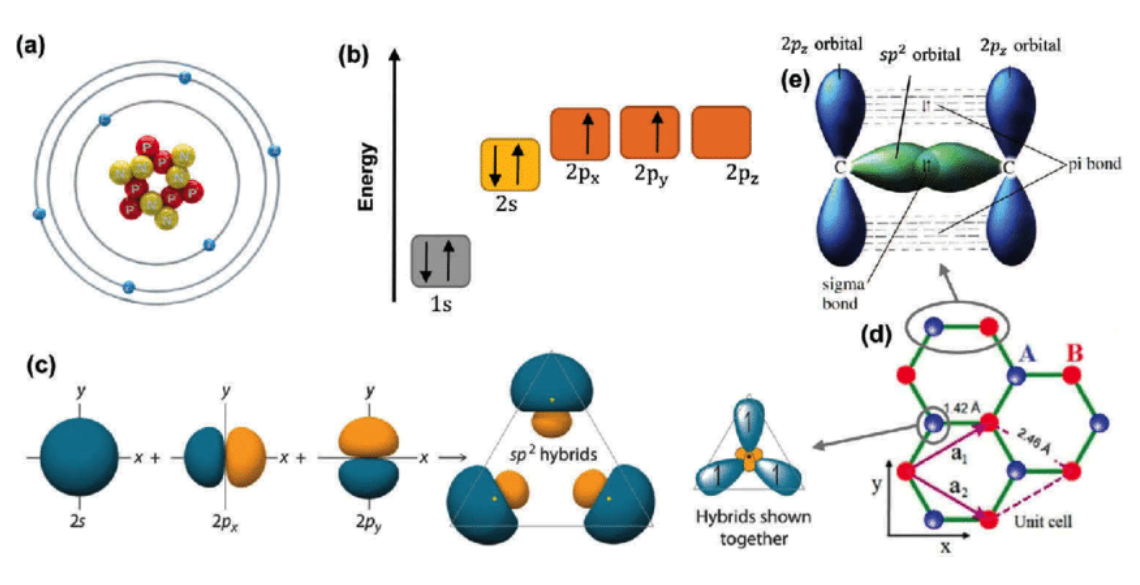
\includegraphics[width=0.479\textwidth]{Lec25/3p2 Hybridization}
    \caption{$sp^2$ Hybridization}
\end{figure}
